% This is based on "sig-alternate.tex" V1.9 April 2009
% This file should be compiled with V2.4 of "sig-alternate.cls" April 2009
%
\documentclass{report}

\usepackage[english]{babel}
\usepackage{graphicx}
\usepackage{tabularx}
\usepackage{subfigure}
\usepackage{enumitem}
\usepackage{url}


\usepackage{color}
\definecolor{orange}{rgb}{1,0.5,0}
\definecolor{lightgray}{rgb}{.9,.9,.9}
\definecolor{java_keyword}{rgb}{0.37, 0.08, 0.25}
\definecolor{java_string}{rgb}{0.06, 0.10, 0.98}
\definecolor{java_comment}{rgb}{0.12, 0.38, 0.18}
\definecolor{java_doc}{rgb}{0.25,0.35,0.75}

% code listings

\usepackage{listings}
\lstloadlanguages{Java}
\lstset{
	language=Java,
	basicstyle=\scriptsize\ttfamily,
	backgroundcolor=\color{lightgray},
	keywordstyle=\color{java_keyword}\bfseries,
	stringstyle=\color{java_string},
	commentstyle=\color{java_comment},
	morecomment=[s][\color{java_doc}]{/**}{*/},
	tabsize=2,
	showtabs=false,
	extendedchars=true,
	showstringspaces=false,
	showspaces=false,
	breaklines=true,
	numbers=left,
	numberstyle=\tiny,
	numbersep=6pt,
	xleftmargin=3pt,
	xrightmargin=3pt,
	framexleftmargin=3pt,
	framexrightmargin=3pt,
	captionpos=b
}

% Disable single lines at the start of a paragraph (Schusterjungen)

\clubpenalty = 10000

% Disable single lines at the end of a paragraph (Hurenkinder)

\widowpenalty = 10000
\displaywidowpenalty = 10000
 
% allows for colored, easy-to-find todos

\newcommand{\todo}[1]{\textsf{\textbf{\textcolor{orange}{[[#1]]}}}}

% consistent references: use these instead of \label and \ref

\newcommand{\lsec}[1]{\label{sec:#1}}
\newcommand{\lssec}[1]{\label{ssec:#1}}
\newcommand{\lfig}[1]{\label{fig:#1}}
\newcommand{\ltab}[1]{\label{tab:#1}}
\newcommand{\rsec}[1]{Section~\ref{sec:#1}}
\newcommand{\rssec}[1]{Section~\ref{ssec:#1}}
\newcommand{\rfig}[1]{Figure~\ref{fig:#1}}
\newcommand{\rtab}[1]{Table~\ref{tab:#1}}
\newcommand{\rlst}[1]{Listing~\ref{#1}}

% General information

\title{Multiplayer Pacman\\
\normalsize{Distributed Systems -- Project Proposal}}
\subtitle{subtitle}

% Use the \alignauthor commands to handle the names
% and affiliations for an 'aesthetic maximum' of six authors.

\numberofauthors{1} %  in this sample file, there are a *total*
% of EIGHT authors. SIX appear on the 'first-page' (for formatting
% reasons) and the remaining two appear in the \additionalauthors section.
%
\author{
% You can go ahead and credit any number of authors here,
% e.g. one 'row of three' or two rows (consisting of one row of three
% and a second row of one, two or three).
%
% The command \alignauthor (no curly braces needed) should
% precede each author name, affiliation/snail-mail address and
% e-mail address. Additionally, tag each line of
% affiliation/address with \affaddr, and tag the
% e-mail address with \email.
%
% 1st. author
\alignauthor \normalsize{Student One,  Student Two, Student Three}\\
	\affaddr{\normalsize{ETH ID-1 XX-XXX-XXX, ETH ID-2 XX-XXX-XXX, ETH ID-3 XX-XXX-XXX}}\\
	\email{\normalsize{one@student.ethz.ch, two@student.ethz.ch, three@student.ethz.ch}}
}


\begin{document}

\maketitle

\begin{abstract}

%--------------------------------------ABSTRACT-------------------------------------


\textit{(a)}~System overview
\textit{(b)}~software and hardware you intend to use in this project,
\textit{(c)}~expected deliveries of this project.
\end{abstract}

\section{Introduction}

%------------------------------------INTRODUCTION------------------------------------



\section{System Overview}

%-----------------------------------SYSTEM OVERVIEW----------------------------------


\begin{figure}[h]
	\centering
    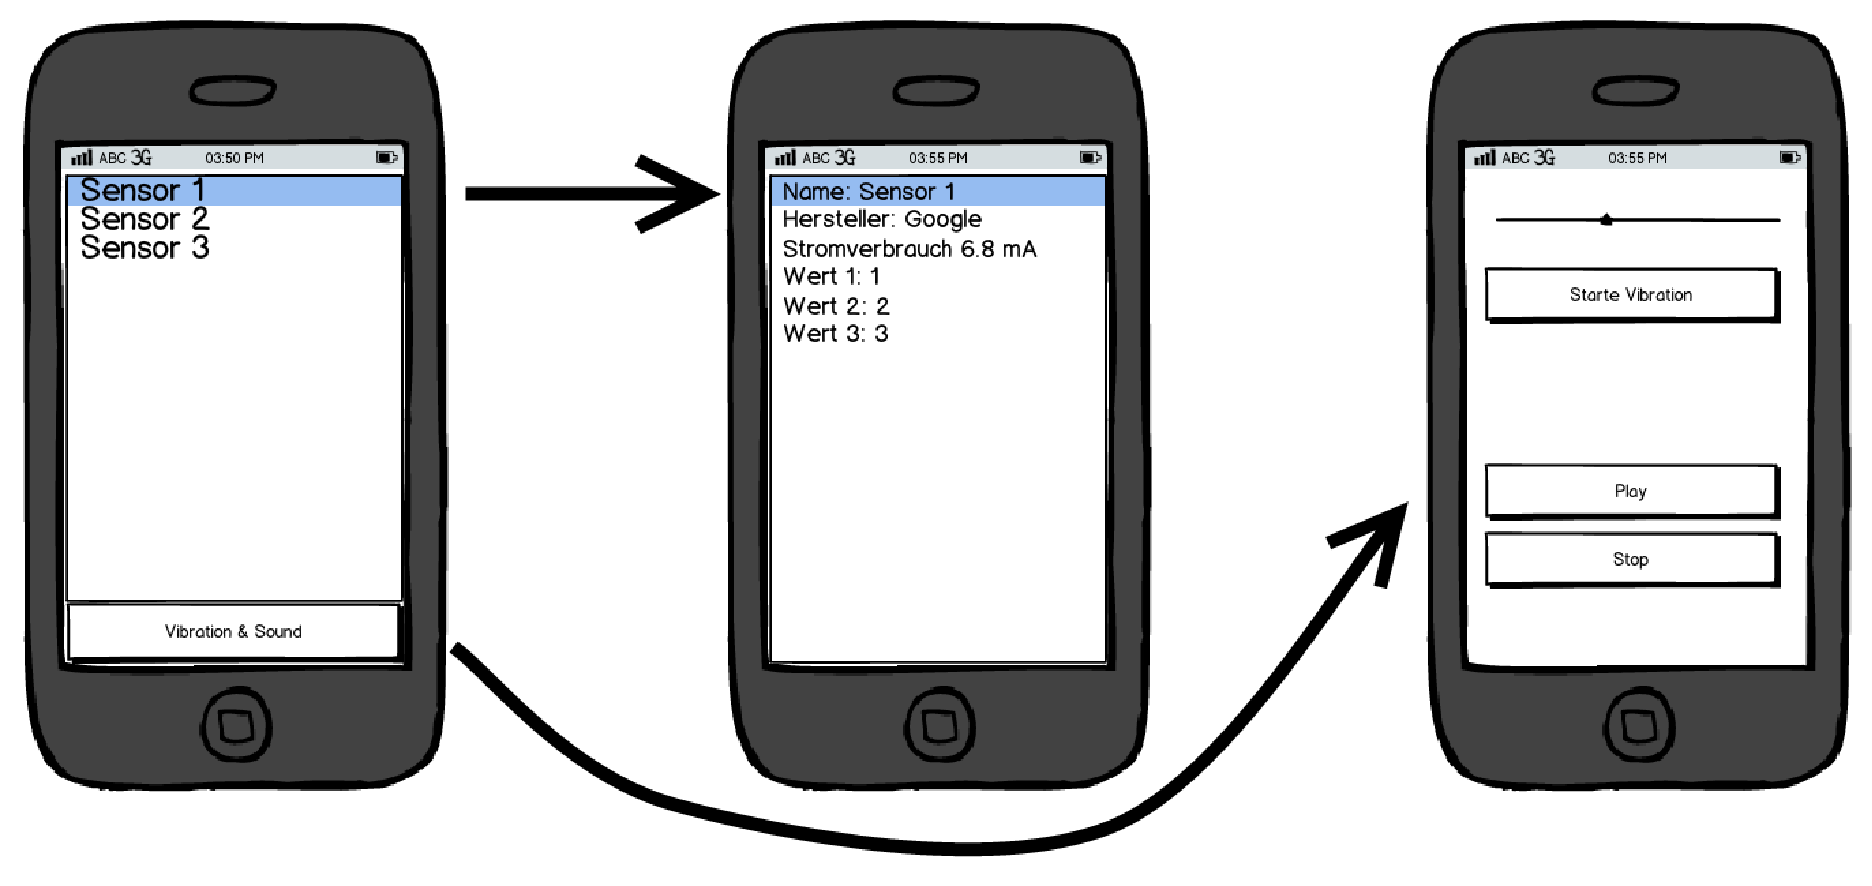
\includegraphics[width=\columnwidth]{example}
    \lfig{example}
    \vspace{-5mm} % use negative white space to fix too large gaps
	\caption{Only include useful figures. Do not simply copy something from a Web.}
\end{figure}



\section{Requirements}

%-------------------------------------REQUIREMENTS------------------------------------

\begin{enumerate}
	\item The game can be played on multiple Android devices.
	\item The gameplay should work as follows:
	\begin{enumerate}
		\item Coins are distributed evenly on the game map (board).
		\item One player plays as PacMan
		\item One or multiple other players play as ghosts
		\item PacMan wins, if he collects all coins on the map
		\item The ghosts win, if they capture PacMan (simply modeled by collision).
	\end{enumerate}
	\item Each player must use one Android device in order to control his figure (PacMan or ghost)
	\item The map (board) on which the players move should provide the following features:
	\begin{enumerate}
		\item PacMan starts on a predefined location (PacMan spawn)
		\item The ghosts (one ore multiple) start on predefined locations (ghost spawns)
		\item Player figures can only move up, down, left and right.
		\item The map is shaped like a maze. ??? [NOT PRECISE ENOUGH]
		\item The only structuring elements of the map are walls.
	\end{enumerate}
	\item The protocol used for Device-to-Device communication will will be implemented atop UDP, TCP or a higher-level protocol [???]
	\item The app will be optimized for Android version [???] and run on Android version [???] and higher. [???]
	\item The player who hosts the game will also play as PacMan.
	\item On the hosting player's device, a server task will be started that clients can connect to. 
	\item The players that connect to a hosted game play as ghosts.
	
\end{enumerate}

The Project 

\begin{figure}[h]
	\centering
    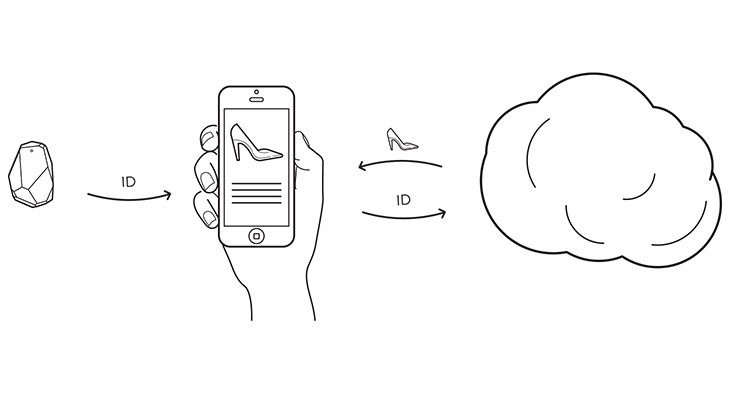
\includegraphics[width=\columnwidth]{overview.jpg}
    \lfig{system-overview}
    \vspace{-5mm} % use negative white space to fix too large gaps
	\caption{System Overview~\cite{estimote}}
\end{figure}

\section{Work Packages}

%-----------------------------------WORK PACKAGES----------------------------------

\begin{itemize}
        \item {\bf WP1}:  XYZ  \ldots    
        \item {\bf WP2}: Set and Configuring Backend Serve  \ldots    
        \item {\bf WP3}: Integration  \ldots 
         \item {\bf WPx}:  \ldots 
\end{itemize}
 
Stick to a concise, scientific writing style. 

\section{Milestones}

%-------------------------------------REFERENCES-----------------------------------

% The following two commands are all you need in the
% initial runs of your .tex file to
% produce the bibliography for the citations in your paper.
\bibliographystyle{abbrv}
\bibliography{report}  % sigproc.bib is the name of the Bibliography in this case
% You must have a proper ".bib" file

%\balancecolumns % GM June 2007

\end{document}
